\documentclass{article}
\usepackage[a4paper, total={7in, 9.5in}]{geometry}
\usepackage{amsmath,amsfonts,amsthm,amssymb,graphicx,float, setspace, bm}
\usepackage[utf8]{inputenc}
\usepackage{float}
\usepackage{titlesec}
\usepackage{setspace}
\usepackage{geometry}
\usepackage[style=numeric]{biblatex}
\usepackage[autostyle=true]{csquotes}
\usepackage{breqn}
\usepackage{subfig}
\usepackage[bottom]{footmisc}
\usepackage{adjustbox}
\usepackage{lipsum}
\usepackage{hyperref}
\usepackage[ruled,vlined]{algorithm2e}
\hypersetup{
    colorlinks=true,
    urlcolor=magenta
}
\usepackage[table,x11names]{xcolor}

\usepackage{xltabular}
\usepackage{multirow}
\usepackage{booktabs}


\renewcommand{\baselinestretch}{1.5} 
\setlength\parindent{0pt}
%----------------------------------------------------------------------------------------
%	START
%----------------------------------------------------------------------------------------

\newcommand{\horrule}[1]{\rule{\linewidth}{#1}}

\title{ \normalfont \normalsize 
\huge CPSC 532 - Homework 2}
\date{}
\author{Xiaoxuan Liang - 48131163}
\def\cond{\; | \;}

\begin{document}

\maketitle

\begin{enumerate}
\item Evaluation-based Sampling:
\begin{enumerate}
\item Program 1): in 1000 samplings from this program,  each return value is a numeric number estimating mean. Therefore, 1000 samplings return an array of length 1000 overall.
\begin{figure}[!htp]
	\centering
	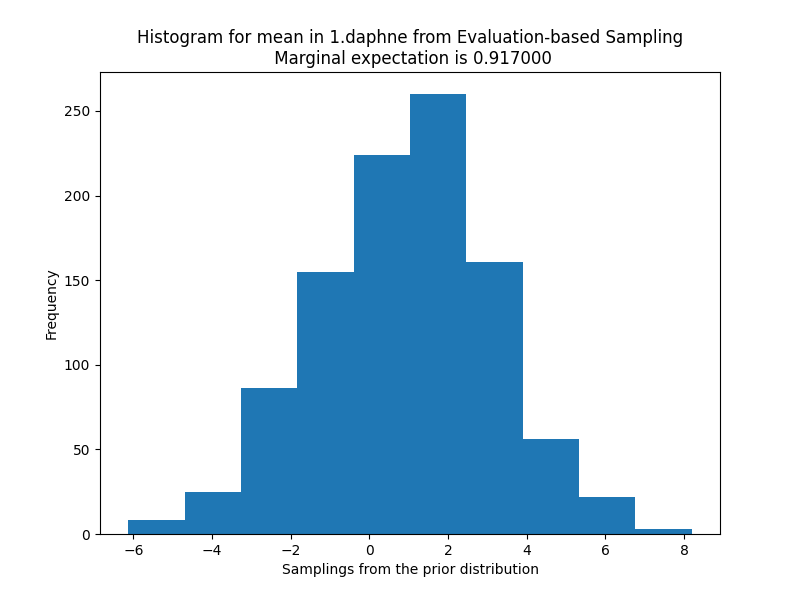
\includegraphics[scale=0.4]{../figs/evaluation_1.png}
	\caption{Histogram from the prior for mean for 1.daphne}
\end{figure}
\item Program 2): in 1000 samplings from this program,  each return value is an array of length 2,  which incorporates the estimations for both slope and bias. Therefore, 1000 samplings return a 2-D array of size $1000\times 2$ overall.
\begin{figure}[!htp] 
    \centering
    \subfloat[Samples from the prior for slope]{%
        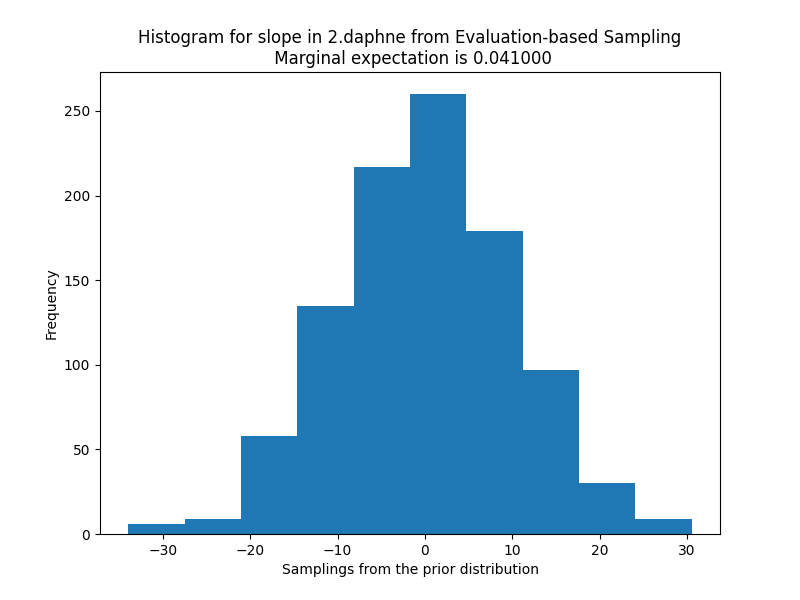
\includegraphics[width=0.4\textwidth]{../figs/evaluation_2_1}%
        \label{fig:a}%
        }%
    \hfill%
    \subfloat[Samples from the prior for bias]{%
        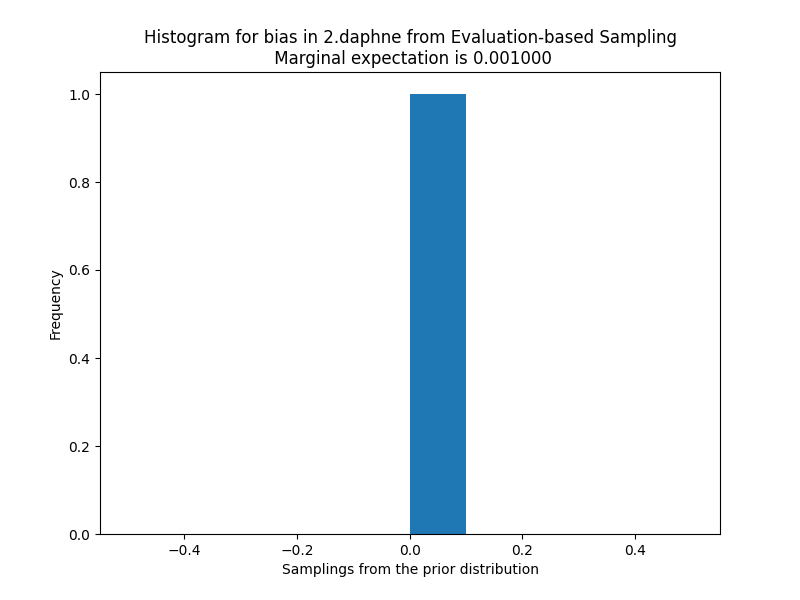
\includegraphics[width=0.4\textwidth]{../figs/evaluation_2_2}%%
        \label{fig:b}%
        }%
        \caption{Histograms for 2.daphne}
\end{figure}

\newpage
\item Program 3): in 1000 samplings from this program, each return value is an array of length 17,  which incorporates the estimations for 17 HMM time steps. Therefore, 1000 sampling returns a 2-D array of size $1000\times 17$ overall.\\
It does not provide statistical meaning for calculating the marginal expectation of the categorical variable, instead,  we can approximate the stationary distribution for the HMM by constructing a $3\times 3$ matrix to record the transition times among all states and calculating the proportion of status of states, which is $\begin{bmatrix}
1506875 & 0.2224375, & 0.626875 
\end{bmatrix}$.
\begin{figure}[!htp]
	\centering
	 \subfloat[Samples from the prior for HMM step 1]{%
        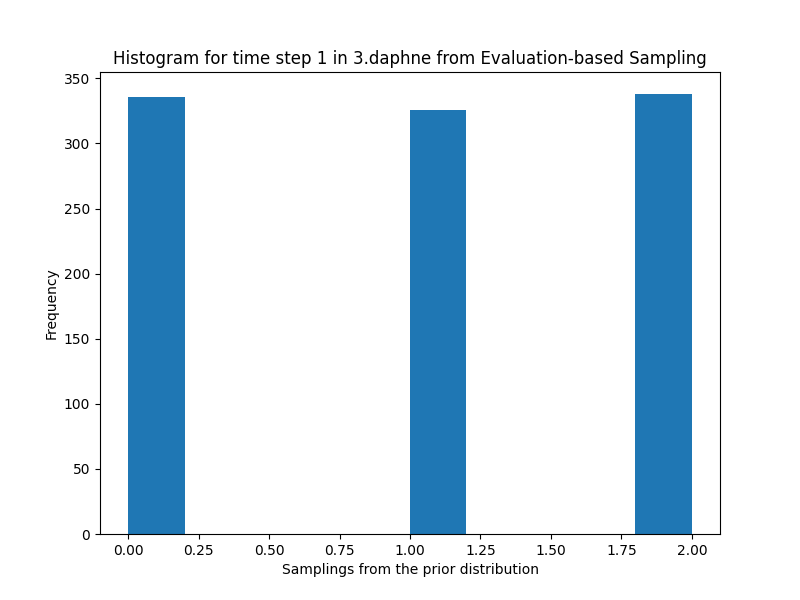
\includegraphics[width=0.2\textwidth]{../figs/evaluation_3_1}%
        \label{fig:a}%
        }%
    \hfill%
    \subfloat[Samples from the prior for HMM step 2]{%
        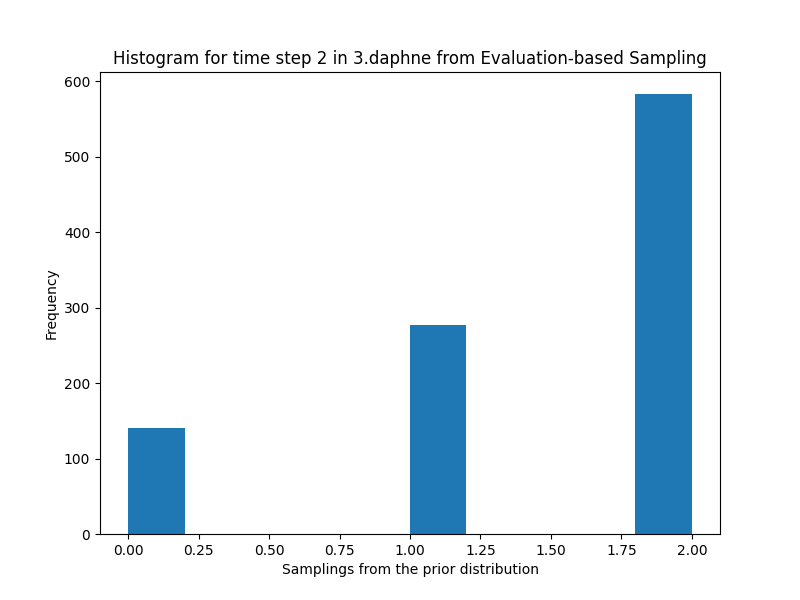
\includegraphics[width=0.2\textwidth]{../figs/evaluation_3_2}%
        \label{fig:b}%
        }%
   \hfill%
   \subfloat[Samples from the prior for HMM step 3]{%
   	  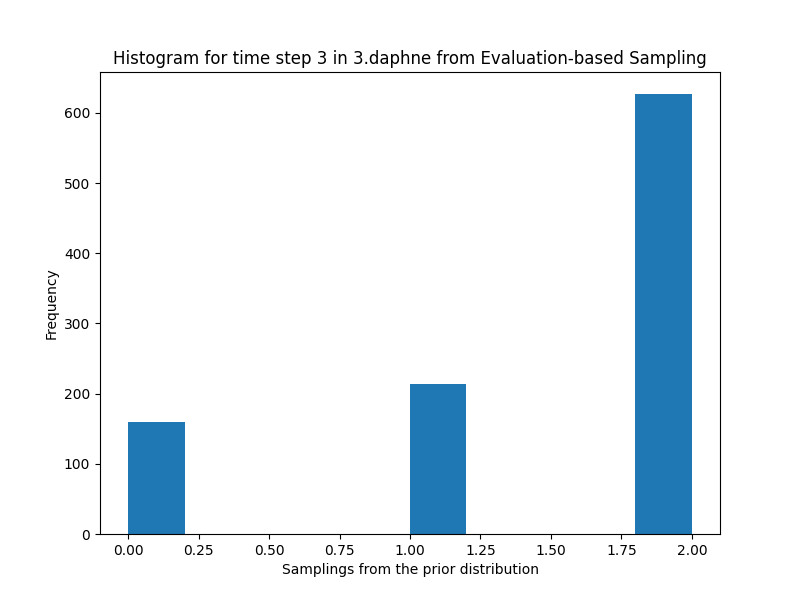
\includegraphics[width=0.2\textwidth]{../figs/evaluation_3_3}%
   	  \label{fig:a}%
   	  }%
   \hfill%
	 \subfloat[Samples from the prior for HMM step 4]{%
        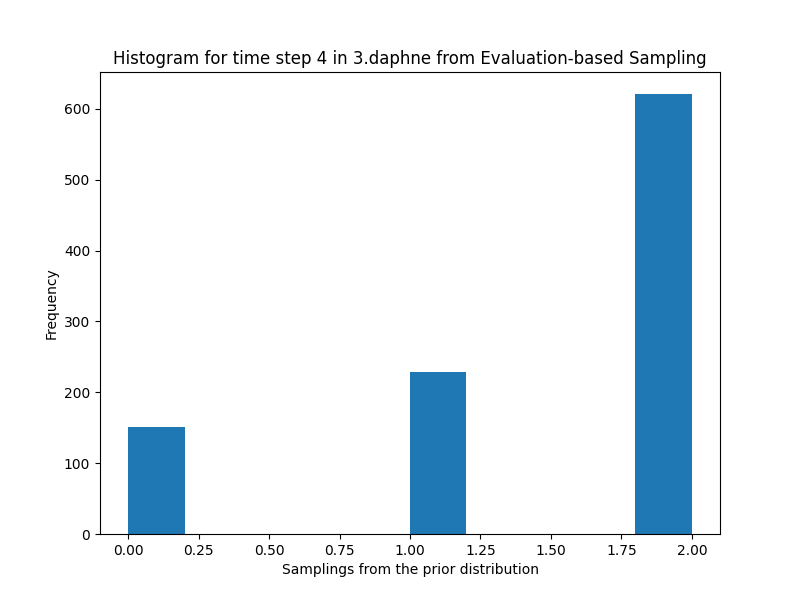
\includegraphics[width=0.2\textwidth]{../figs/evaluation_3_4}%
        \label{fig:d}%
        }%
        
   \hfill%
    \subfloat[Samples from the prior for HMM step 5]{%
        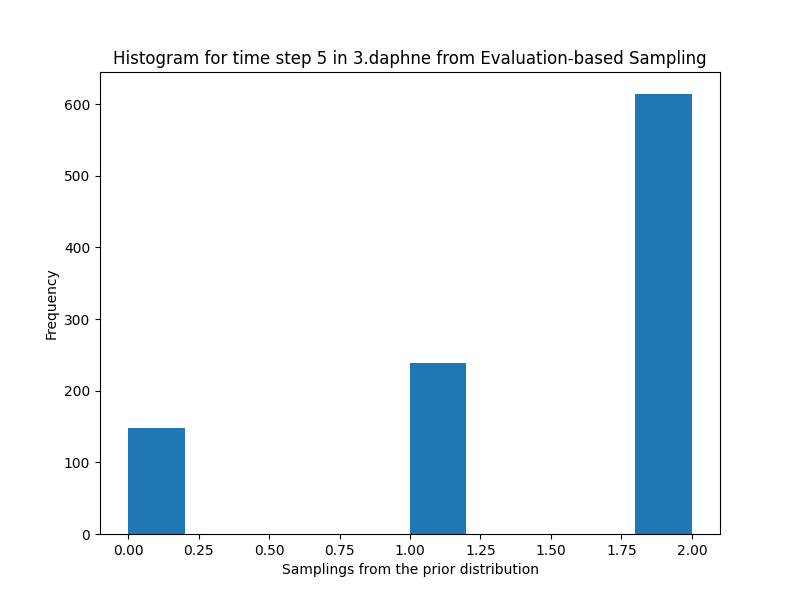
\includegraphics[width=0.24\textwidth]{../figs/evaluation_3_5}%
        \label{fig:e}%
        }%
   \centering
   \subfloat[Samples from the prior for HMM step 6]{%
   	  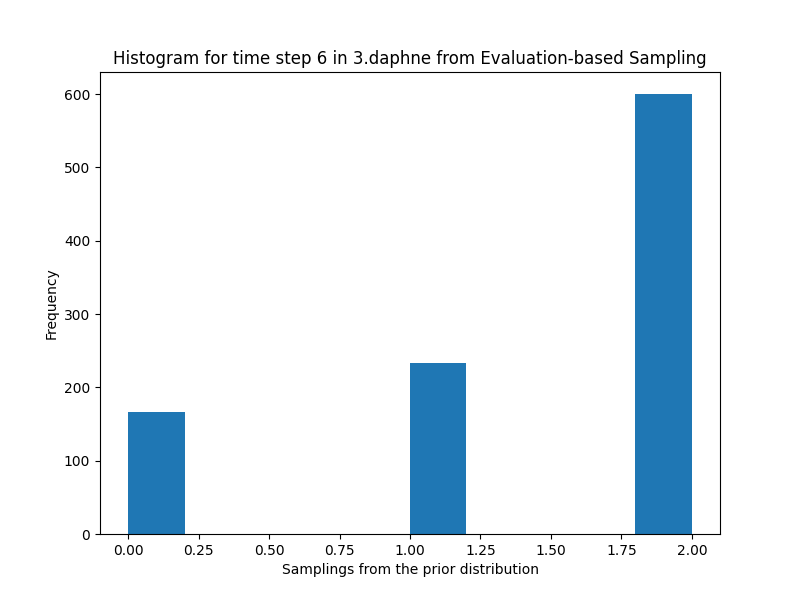
\includegraphics[width=0.24\textwidth]{../figs/evaluation_3_6}%
   	  \label{fig:f}%
   	  }%
   \hfill%
	 \subfloat[Samples from the prior for HMM step 7]{%
        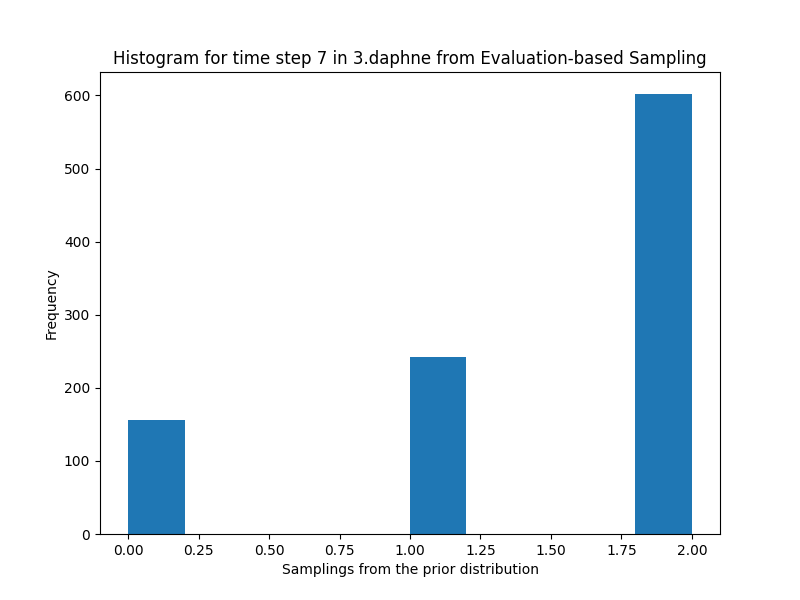
\includegraphics[width=0.24\textwidth]{../figs/evaluation_3_7}%
        \label{fig:d}%
        }%
   \hfill%
    \subfloat[Samples from the prior for HMM step 8]{%
        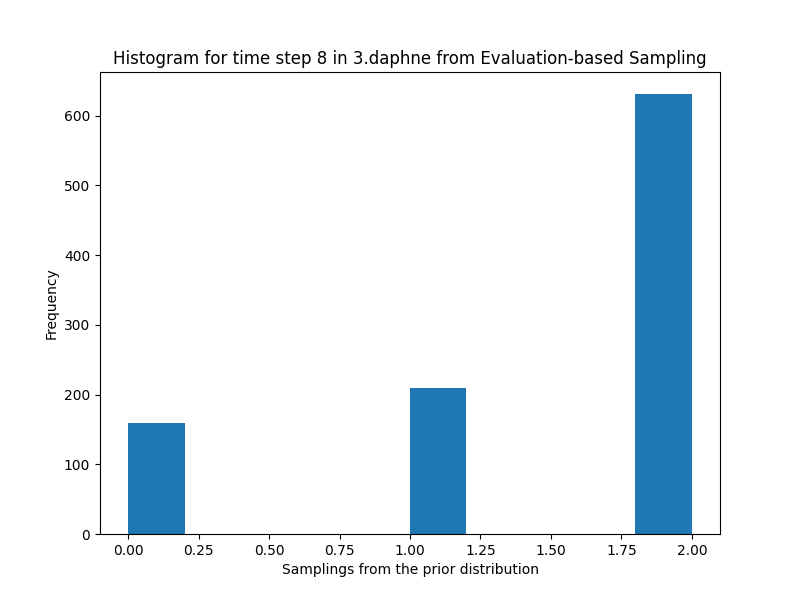
\includegraphics[width=0.24\textwidth]{../figs/evaluation_3_8}%
        \label{fig:e}%
        }%
        
   \centering
   \subfloat[Samples from the prior for HMM step 9]{%
   	  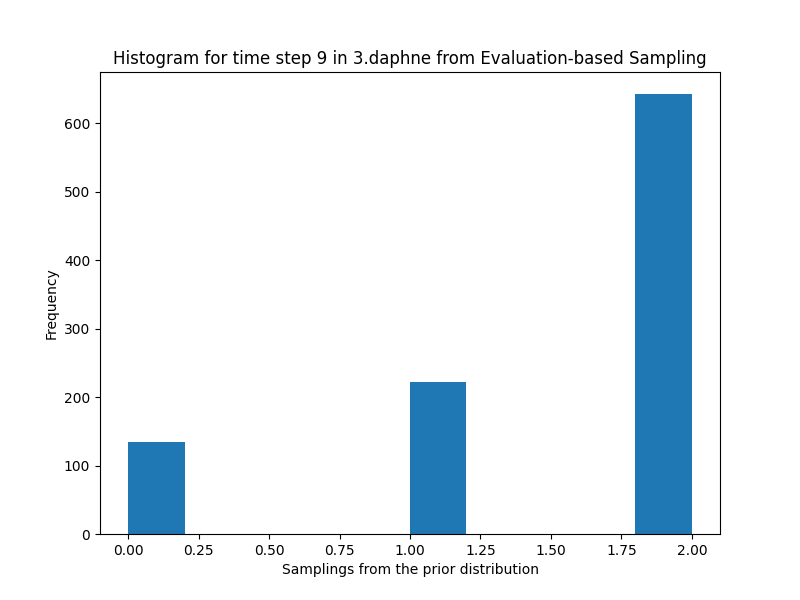
\includegraphics[width=0.24\textwidth]{../figs/evaluation_3_9}%
   	  \label{fig:f}%
   	  }%
   \hfill%
   	  \subfloat[Samples from the prior for HMM step 10]{%
        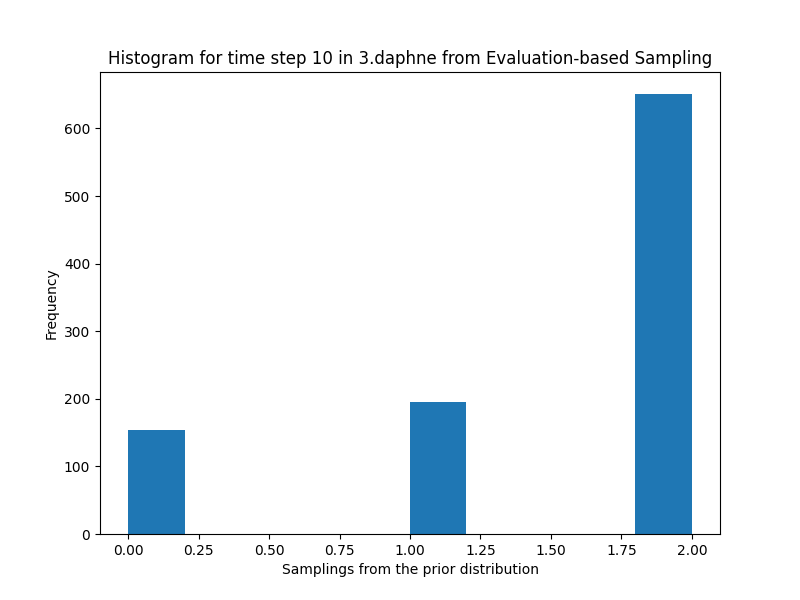
\includegraphics[width=0.24\textwidth]{../figs/evaluation_3_10}%
        \label{fig:d}%
        }%
    \hfill%
    \subfloat[Samples from the prior for HMM step 11]{%
        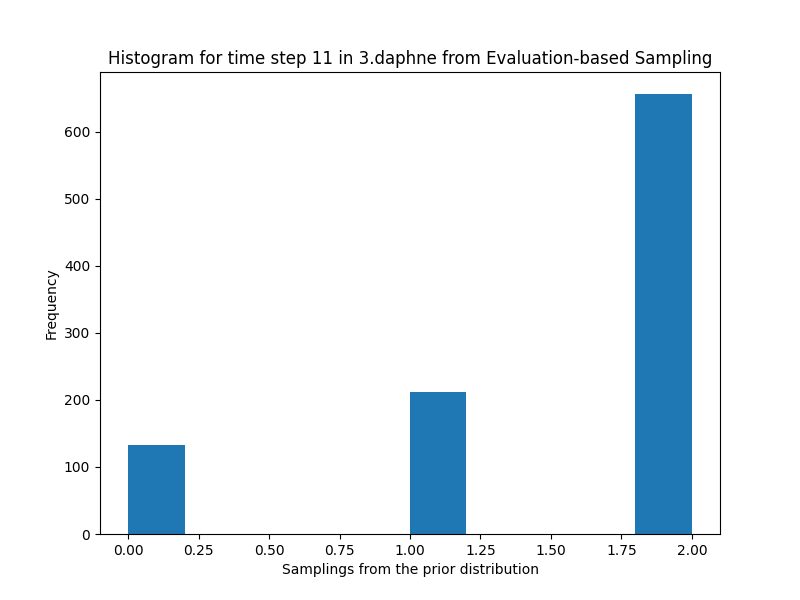
\includegraphics[width=0.24\textwidth]{../figs/evaluation_3_11}%
        \label{fig:e}%
        }%
   \hfill%
   \subfloat[Samples from the prior for HMM step 12]{%
   	  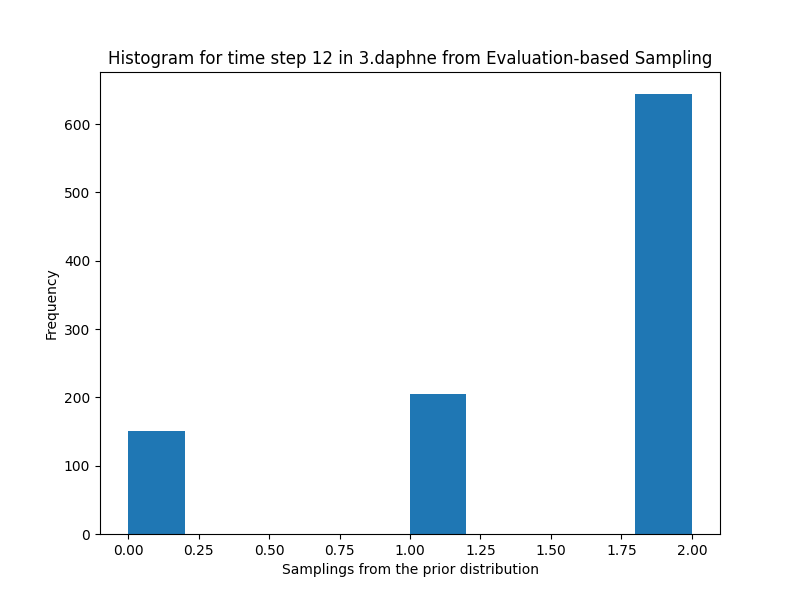
\includegraphics[width=0.24\textwidth]{../figs/evaluation_3_12}%
   	  \label{fig:f}%
   	  }%
   	  
  \centering
   \subfloat[Samples from the prior for HMM step 13]{%
   	  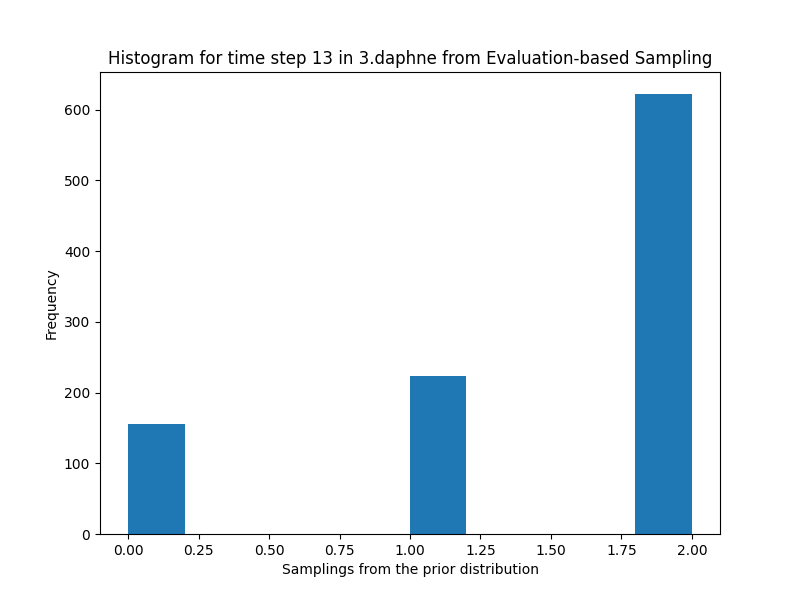
\includegraphics[width=0.24\textwidth]{../figs/evaluation_3_13}%
   	  \label{fig:f}%
   	  }%
   \hfill%
   	  \subfloat[Samples from the prior for HMM step 14]{%
        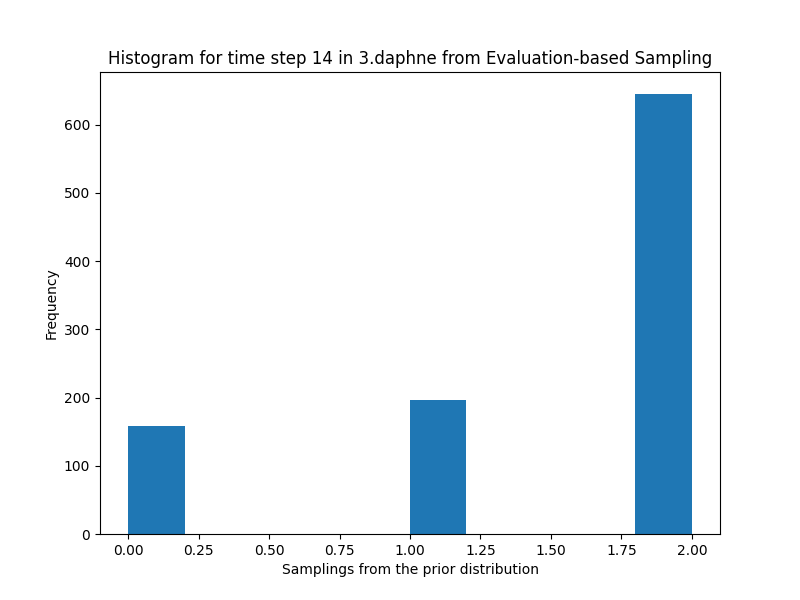
\includegraphics[width=0.24\textwidth]{../figs/evaluation_3_14}%
        \label{fig:d}%
        }%
    \hfill%
    \subfloat[Samples from the prior for HMM step 15]{%
        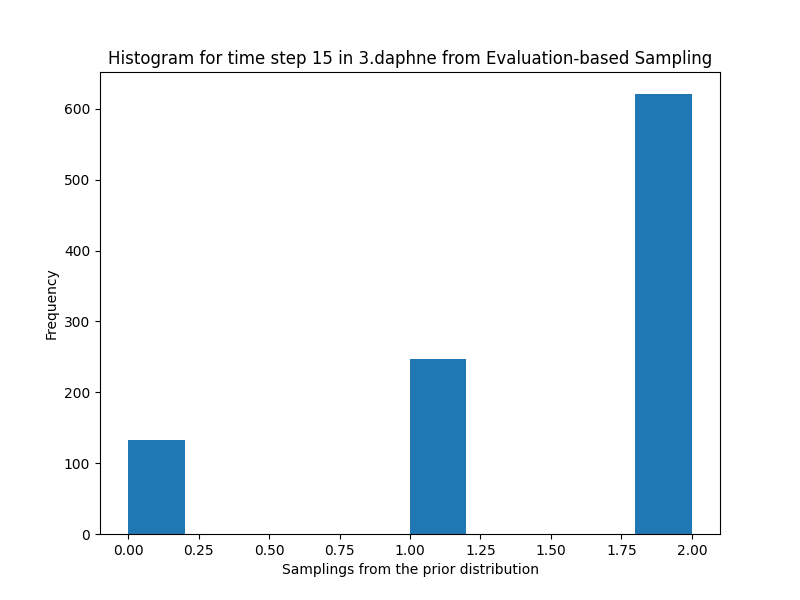
\includegraphics[width=0.24\textwidth]{../figs/evaluation_3_15}%
        \label{fig:e}%
        }%
   \hfill%
   \subfloat[Samples from the prior for HMM step 16]{%
   	  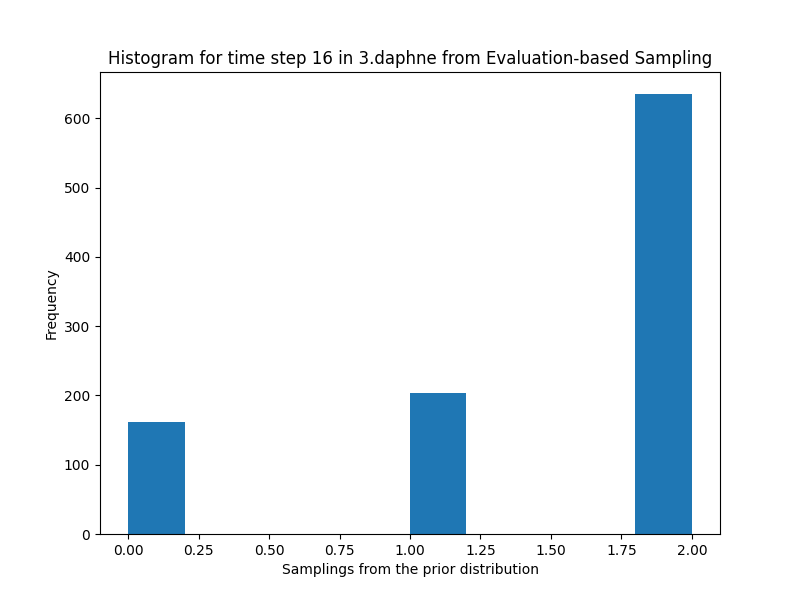
\includegraphics[width=0.24\textwidth]{../figs/evaluation_3_16}%
   	  \label{fig:f}%
   	  }%
  \caption{Partial Histograms for 3.daphne}
\end{figure}

\begin{figure}[!htp]
   \subfloat[Samples from the prior for HMM step 17]{%
   	   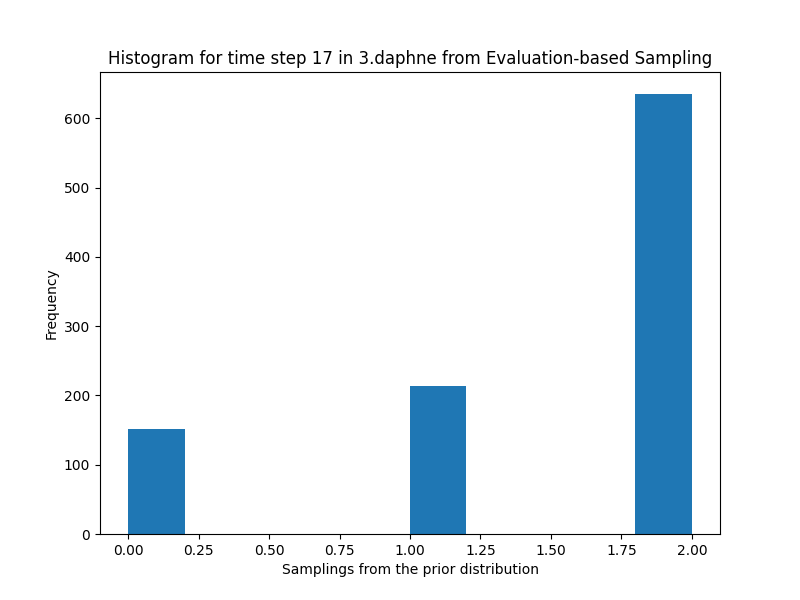
\includegraphics[width=0.24\textwidth]{../figs/evaluation_3_17}%
   	  \label{fig:f}%
   	  }%
   \caption{Histograms for 3.daphne}
\end{figure}

\newpage
\item Program 4): in 1000 samplings from this program,  each return values is a 3-D array incorporating the estimations for $W_0, b_0, W_1, b_1$.  $W_0$ is a 2-D array of size $10\times 1$, $b_0$ is a 2-D array of size $10\times 1$, $W_1$ is a 2-D array of size $10\times 10$, and $b_1$ is a 2-D array of size $10\times 1$.\\
Since all $W_0, b_0, W_1, b_1$ are sampled from standard normal distribution,  I took the mean across the sampled array from each sampling regarded as the resulted sampling, instead of plotting too many histograms.
\begin{figure}[!htp]
	\centering
    \subfloat[Samples from the prior for $W_0$]{%
        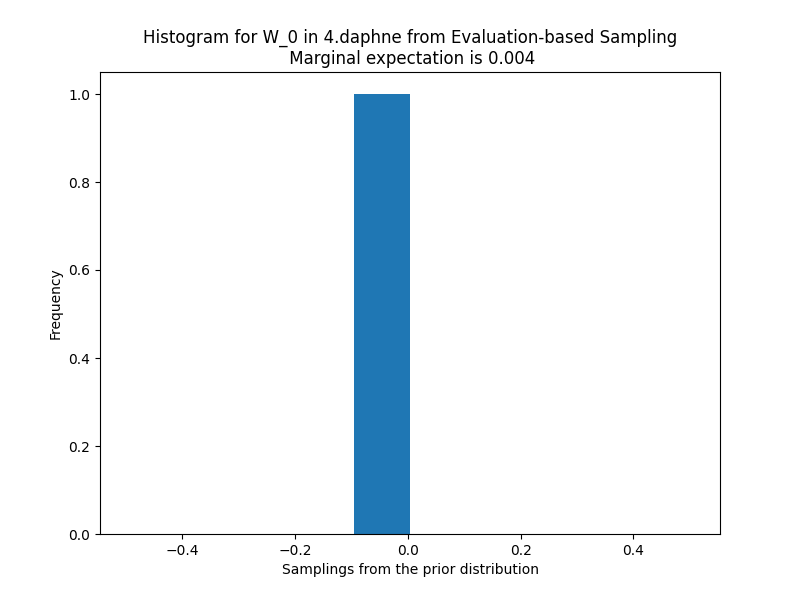
\includegraphics[width=0.4\textwidth]{../figs/evaluation_4_1}%
        \label{fig:a}%
        }%
    \hfill%
    \subfloat[Samples from the prior for $b_0$]{%
        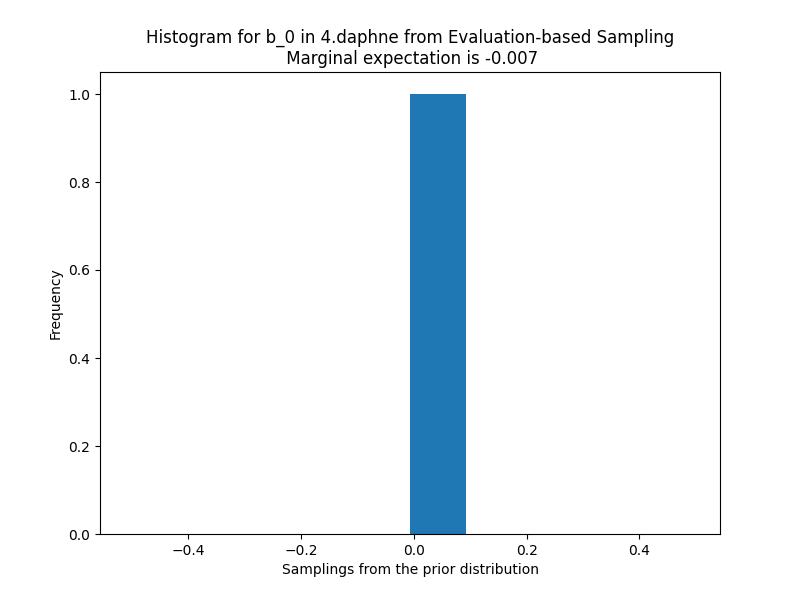
\includegraphics[width=0.4\textwidth]{../figs/evaluation_4_2}%%
        \label{fig:b}%
        }%
	
	\centering
    \subfloat[Samples from the prior for $W_1$]{%
        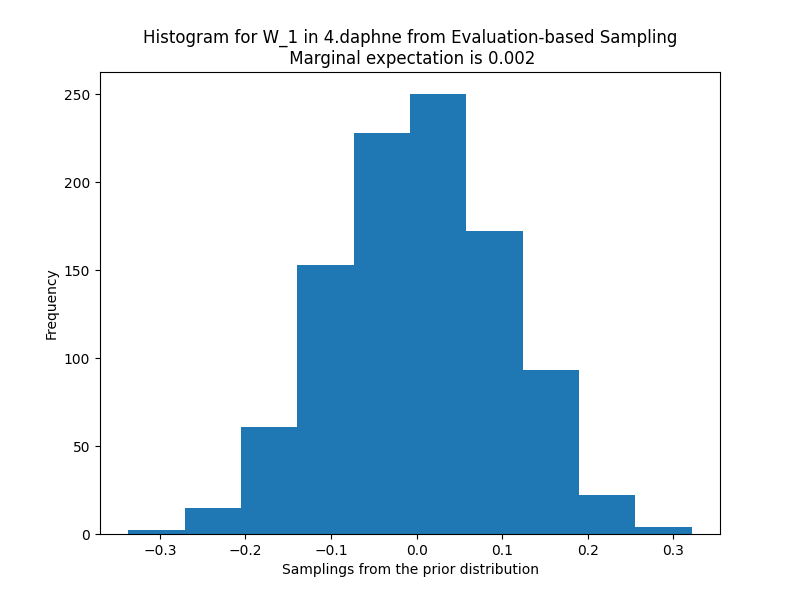
\includegraphics[width=0.4\textwidth]{../figs/evaluation_4_3}%
        \label{fig:a}%
        }%
    \hfill%
    \subfloat[Samples from the prior for $b_1$]{%
        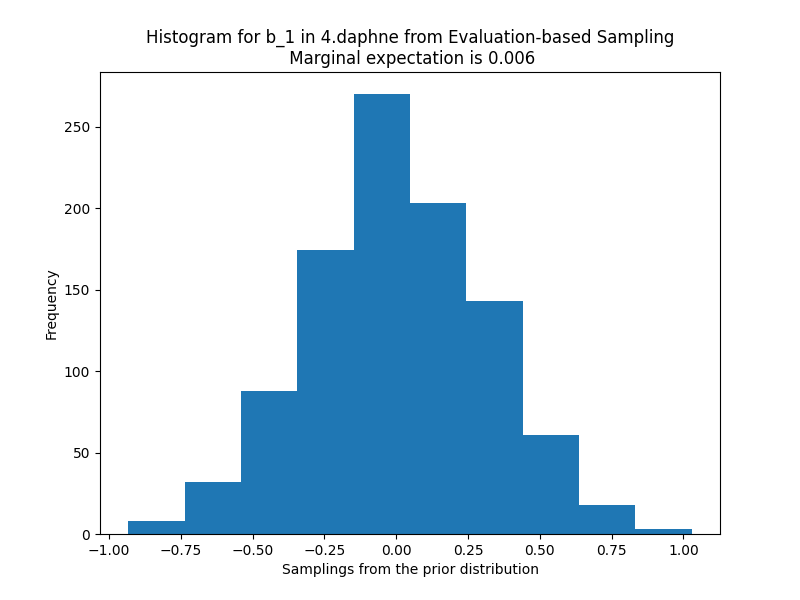
\includegraphics[width=0.4\textwidth]{../figs/evaluation_4_4}%%
        \label{fig:b}%
        }%
        \caption{Histograms for 4.daphne}
\end{figure}
\end{enumerate}
\newpage
\item Graph-based Sampling:
\begin{enumerate}
\item Program 1): in 1000 samplings from this program,  each return value is a numeric number estimating mean. Therefore, 1000 samplings return an array of length 1000 overall.
\begin{figure}[!htp]
	\centering
	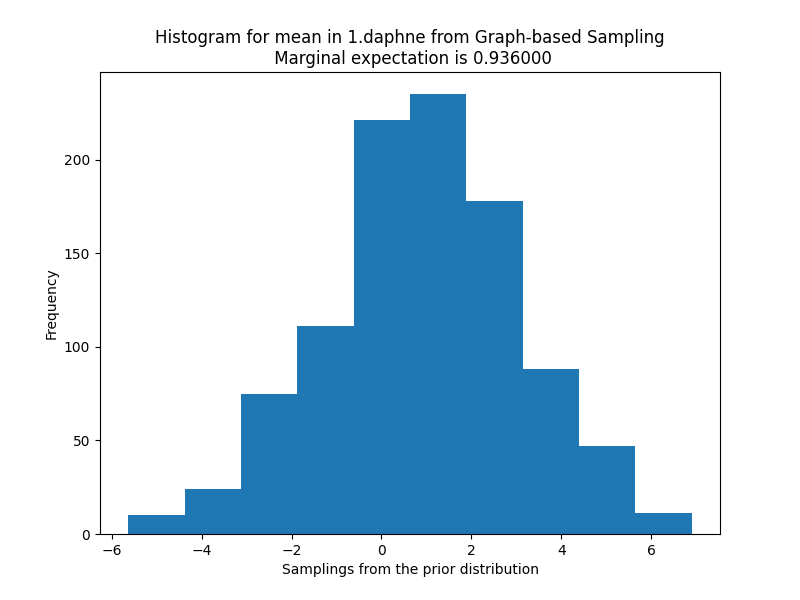
\includegraphics[scale=0.4]{../figs/graph_1.png}
	\caption{Histogram from the prior for mean for 1.daphne}
\end{figure}
\item Program 2): in 1000 samplings from this program,  each return value is an array of length 2,  which incorporates the estimations for both slope and bias. Therefore, 1000 samplings return a 2-D array of size $1000\times 2$ overall.
\begin{figure}[!htp] 
    \centering
    \subfloat[Samples from the prior for slope]{%
        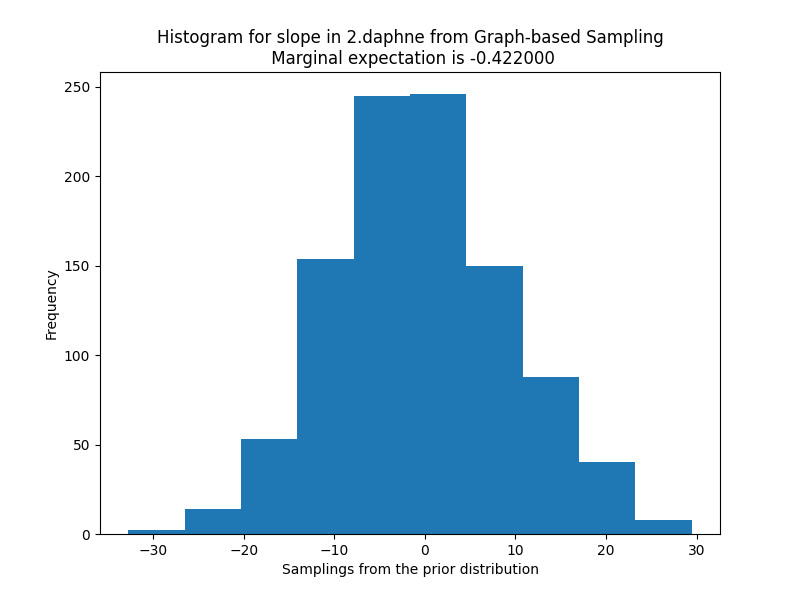
\includegraphics[width=0.4\textwidth]{../figs/graph_2_1}%
        \label{fig:a}%
        }%
    \hfill%
    \subfloat[Samples from the prior for bias]{%
        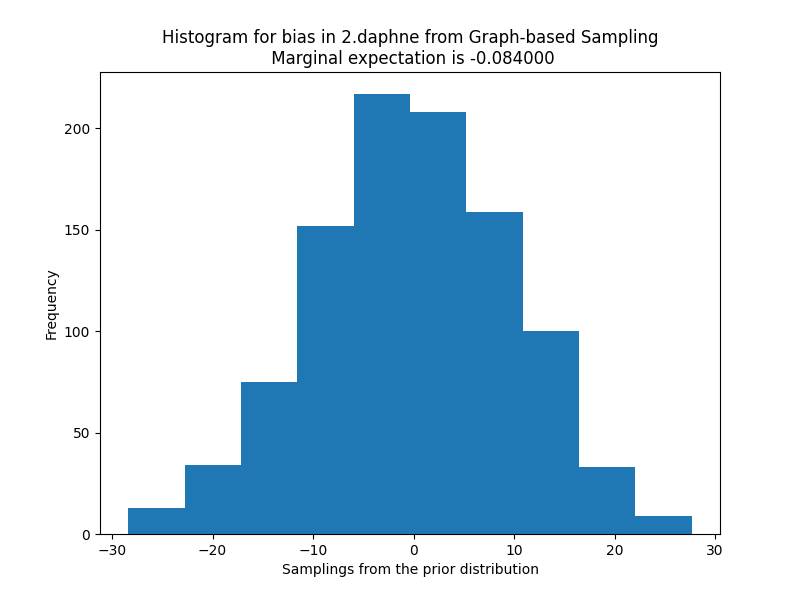
\includegraphics[width=0.4\textwidth]{../figs/graph_2_2}%%
        \label{fig:b}%
        }%
        \caption{Histograms for 2.daphne}
\end{figure}

\newpage
\item Program 3): in 1000 samplings from this program, each return value is an array of length 17,  which incorporates the estimations for 17 HMM time steps. Therefore, 1000 sampling returns a 2-D array of size $1000\times 17$ overall. \\
It does not provide statistical meaning for calculating the marginal expectation of the categorical variable, instead,  we can approximate the stationary distribution for the HMM by constructing a $3\times 3$ matrix to record the transition times among all states and calculating the proportion of status of states, which is $\begin{bmatrix}
0.1550625 & 0.219625 & 0.6253125
\end{bmatrix}$.
\begin{figure}[!htp]
	\centering
	 \subfloat[Samples from the prior for HMM step 1]{%
        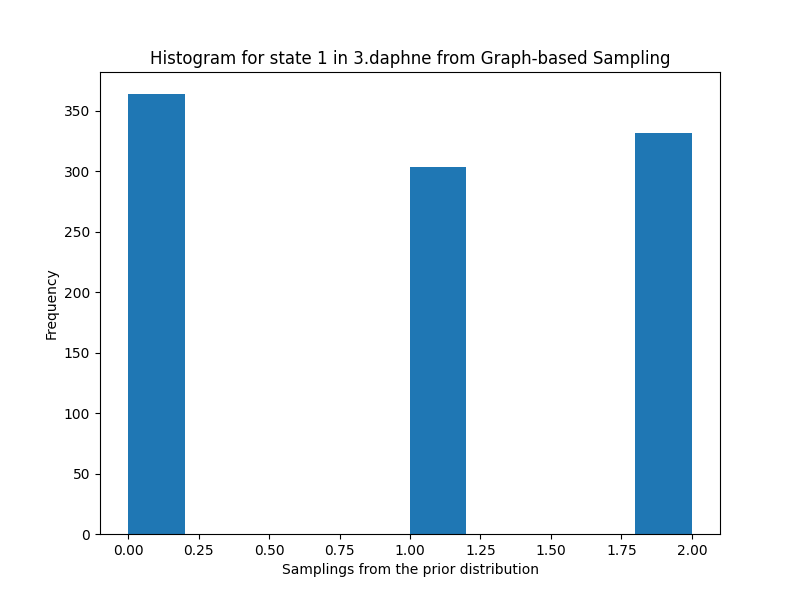
\includegraphics[width=0.2\textwidth]{../figs/graph_3_1}%
        \label{fig:a}%
        }%
    \hfill%
    \subfloat[Samples from the prior for HMM step 2]{%
        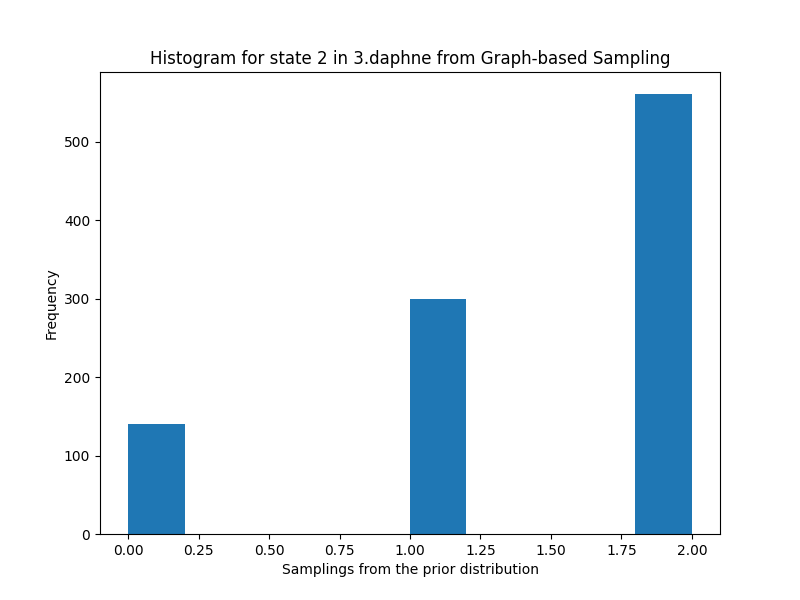
\includegraphics[width=0.2\textwidth]{../figs/graph_3_2}%
        \label{fig:b}%
        }%
   \hfill%
   \subfloat[Samples from the prior for HMM step 3]{%
   	  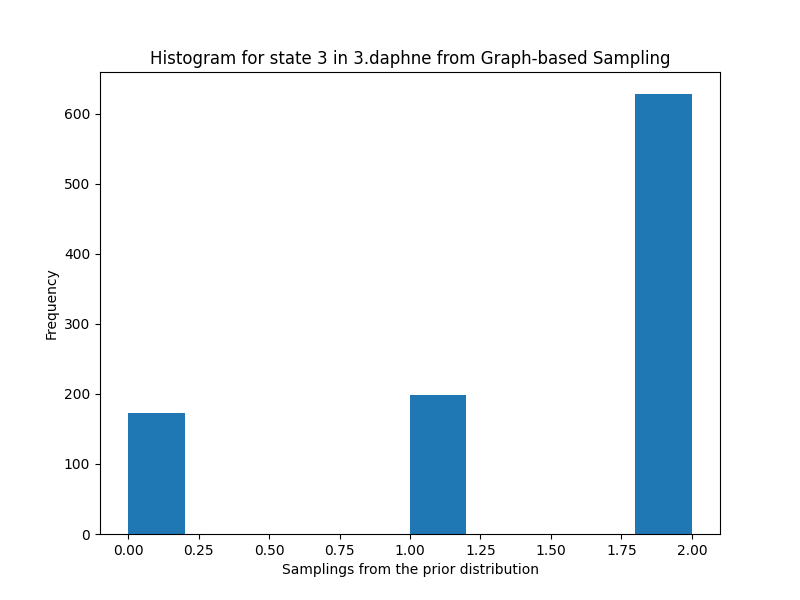
\includegraphics[width=0.2\textwidth]{../figs/graph_3_3}%
   	  \label{fig:a}%
   	  }%
   \hfill%
	 \subfloat[Samples from the prior for HMM step 4]{%
        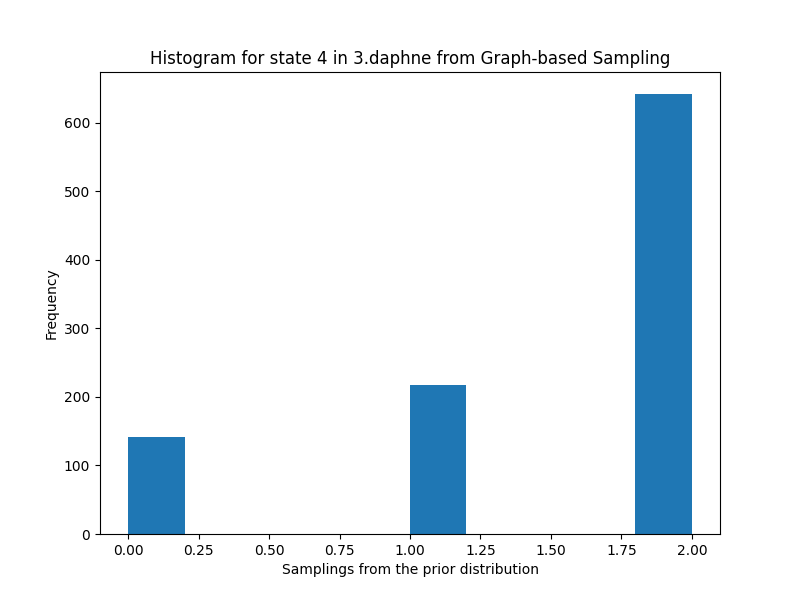
\includegraphics[width=0.2\textwidth]{../figs/graph_3_4}%
        \label{fig:d}%
        }%
        
   \hfill%
    \subfloat[Samples from the prior for HMM step 5]{%
        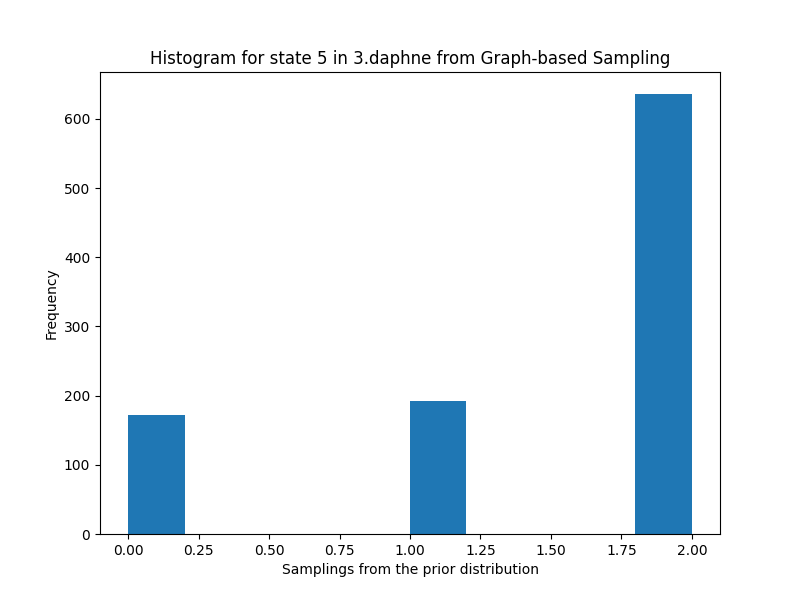
\includegraphics[width=0.24\textwidth]{../figs/graph_3_5}%
        \label{fig:e}%
        }%
   \centering
   \subfloat[Samples from the prior for HMM step 6]{%
   	  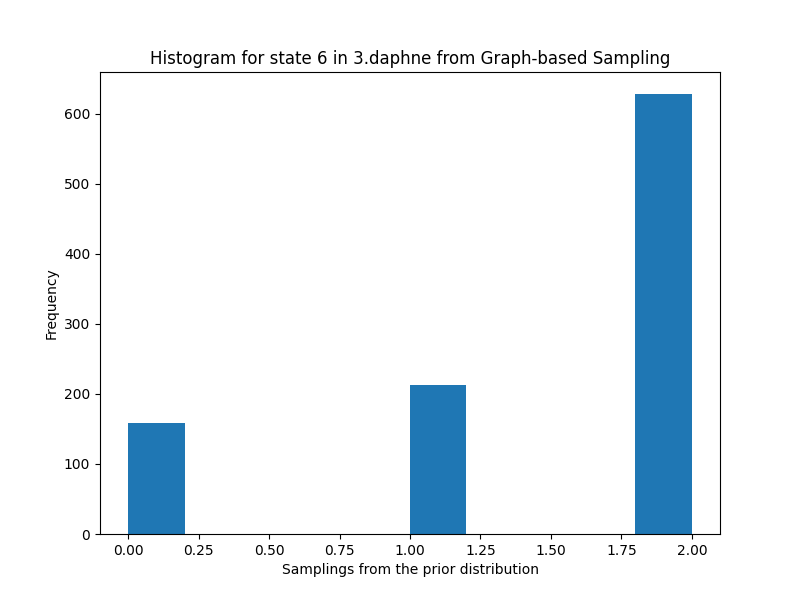
\includegraphics[width=0.24\textwidth]{../figs/graph_3_6}%
   	  \label{fig:f}%
   	  }%
   \hfill%
	 \subfloat[Samples from the prior for HMM step 7]{%
        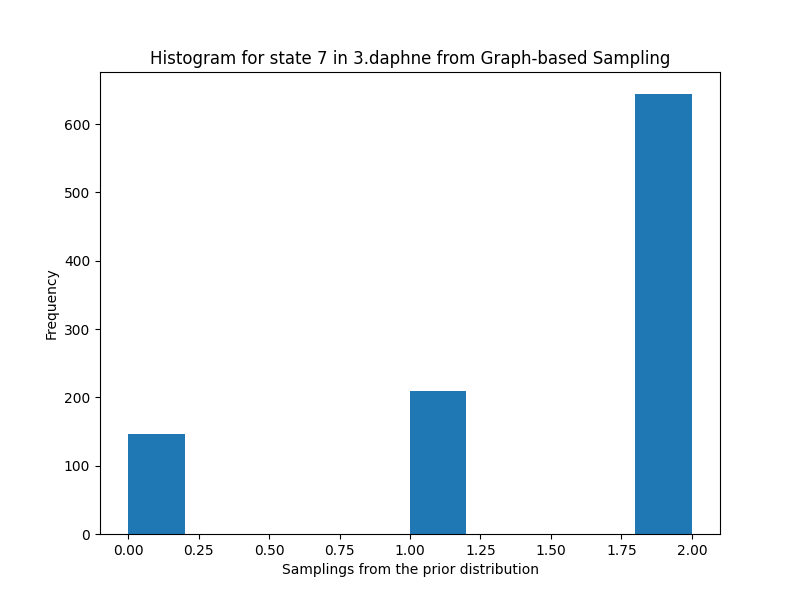
\includegraphics[width=0.24\textwidth]{../figs/graph_3_7}%
        \label{fig:d}%
        }%
   \hfill%
    \subfloat[Samples from the prior for HMM step 8]{%
        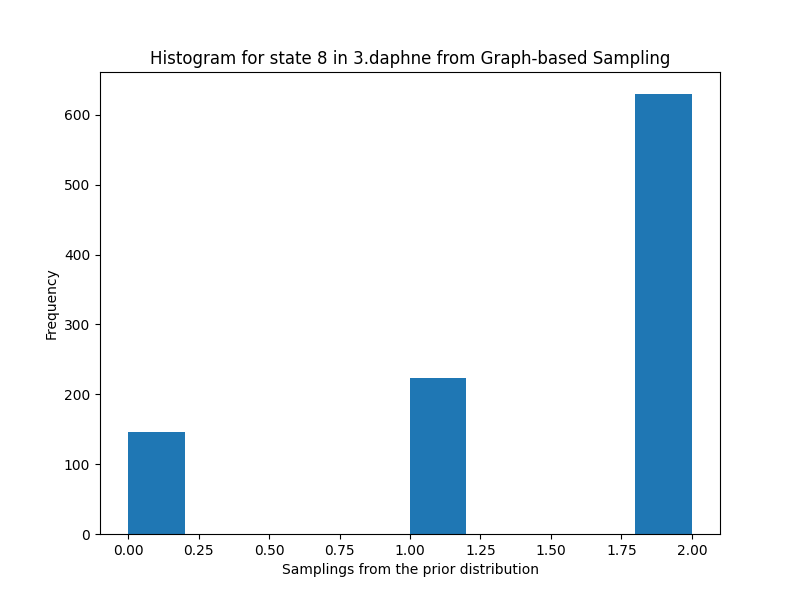
\includegraphics[width=0.24\textwidth]{../figs/graph_3_8}%
        \label{fig:e}%
        }%
        
   \centering
   \subfloat[Samples from the prior for HMM step 9]{%
   	  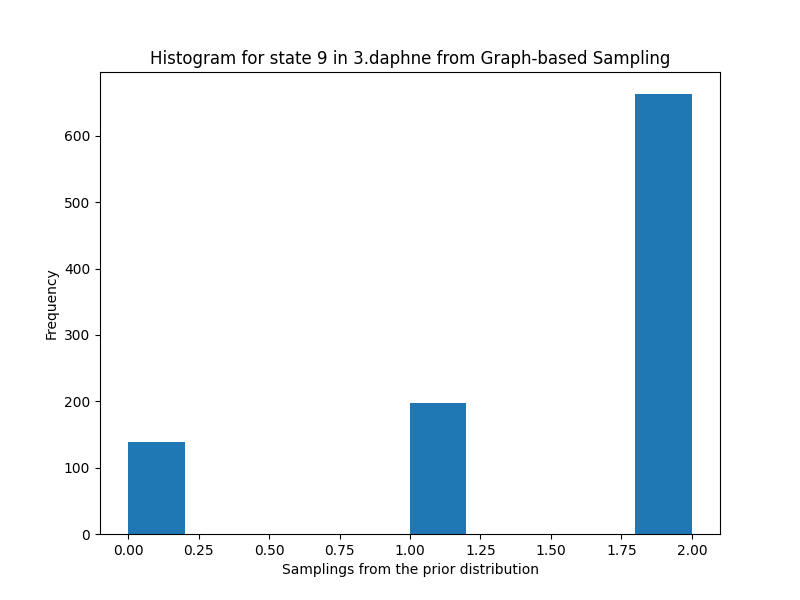
\includegraphics[width=0.24\textwidth]{../figs/graph_3_9}%
   	  \label{fig:f}%
   	  }%
   \hfill%
   	  \subfloat[Samples from the prior for HMM step 10]{%
        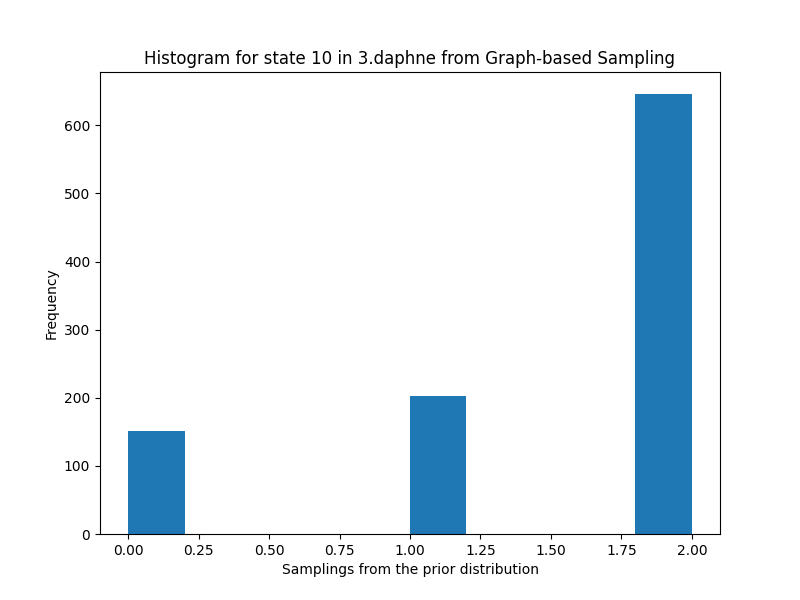
\includegraphics[width=0.24\textwidth]{../figs/graph_3_10}%
        \label{fig:d}%
        }%
    \hfill%
    \subfloat[Samples from the prior for HMM step 11]{%
        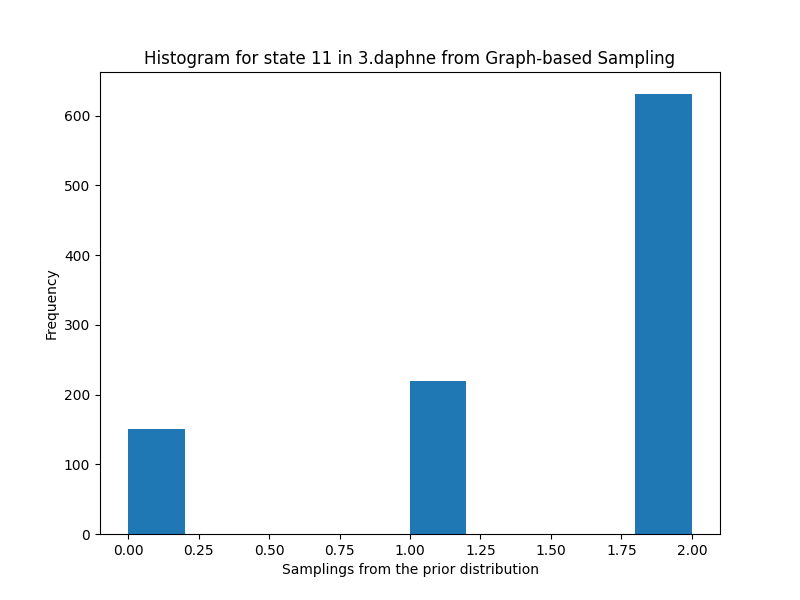
\includegraphics[width=0.24\textwidth]{../figs/graph_3_11}%
        \label{fig:e}%
        }%
   \hfill%
   \subfloat[Samples from the prior for HMM step 12]{%
   	  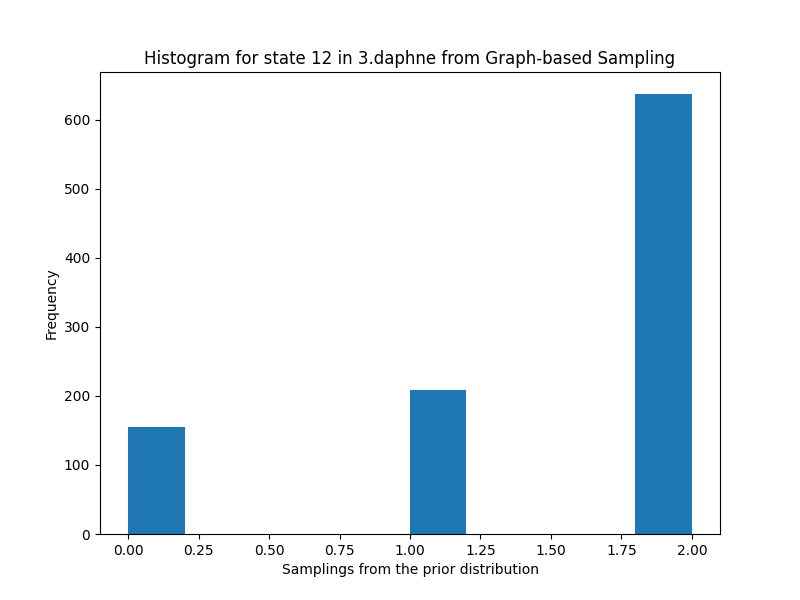
\includegraphics[width=0.24\textwidth]{../figs/graph_3_12}%
   	  \label{fig:f}%
   	  }%
   	  
  \centering
   \subfloat[Samples from the prior for HMM step 13]{%
   	  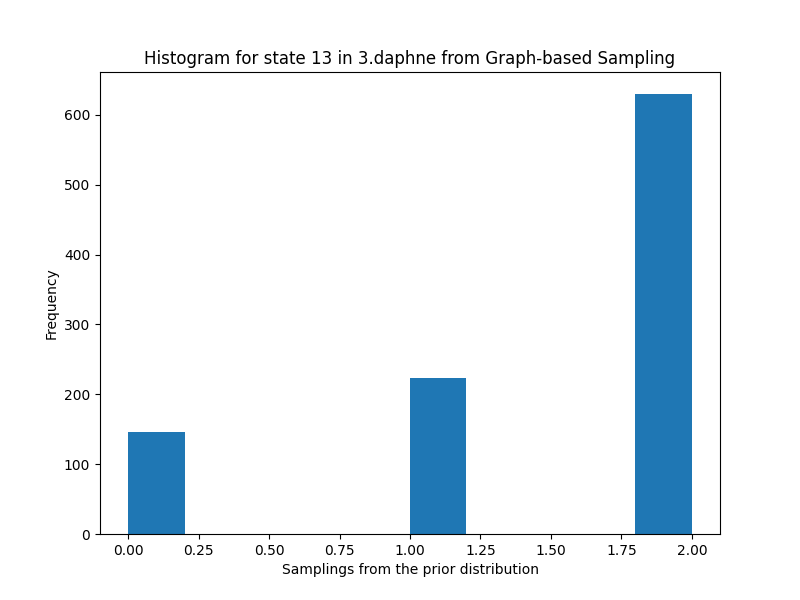
\includegraphics[width=0.24\textwidth]{../figs/graph_3_13}%
   	  \label{fig:f}%
   	  }%
   \hfill%
   	  \subfloat[Samples from the prior for HMM step 14]{%
        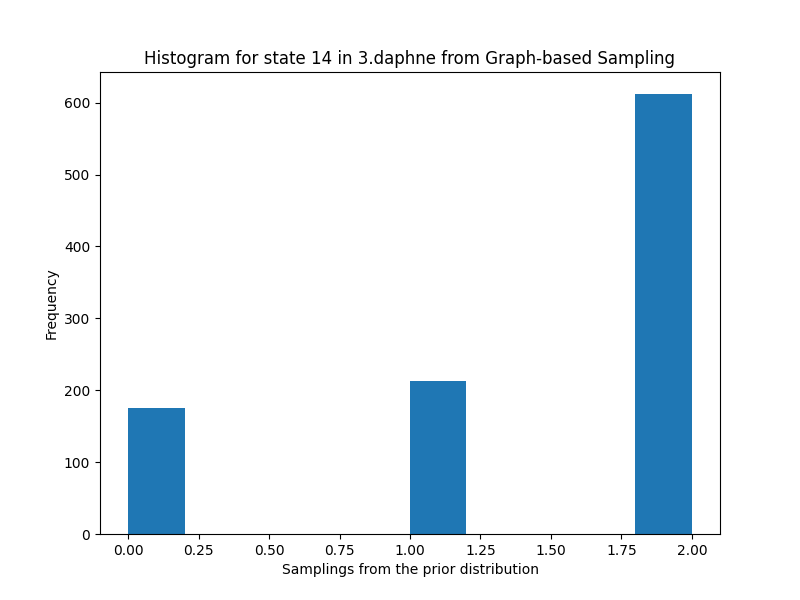
\includegraphics[width=0.24\textwidth]{../figs/graph_3_14}%
        \label{fig:d}%
        }%
    \hfill%
    \subfloat[Samples from the prior for HMM step 15]{%
        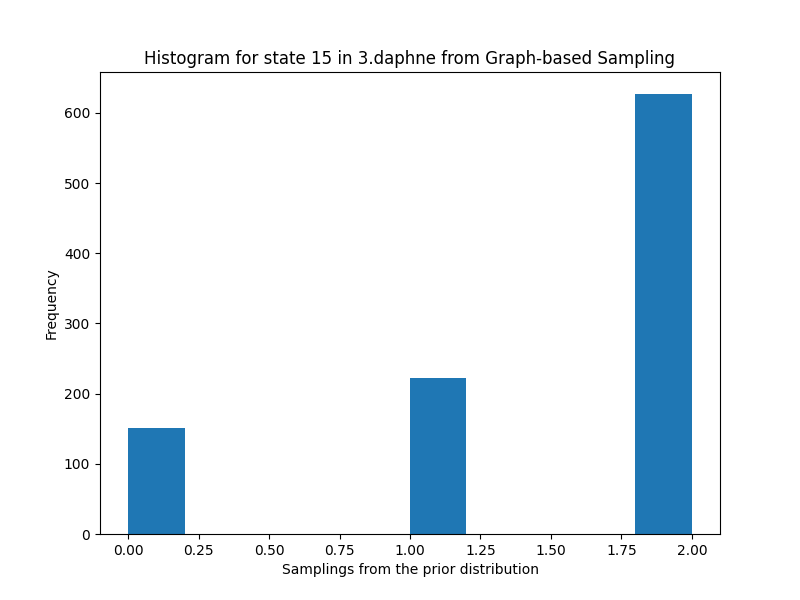
\includegraphics[width=0.24\textwidth]{../figs/graph_3_15}%
        \label{fig:e}%
        }%
   \hfill%
   \subfloat[Samples from the prior for HMM step 16]{%
   	  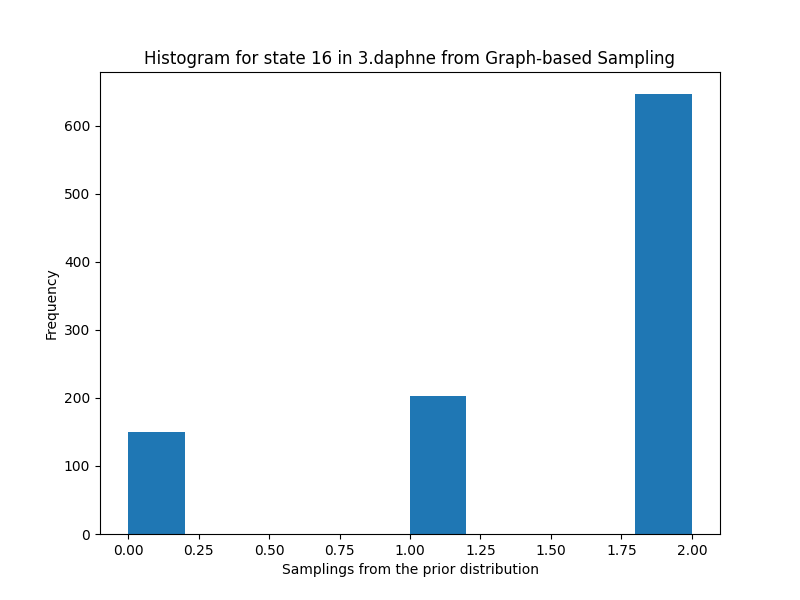
\includegraphics[width=0.24\textwidth]{../figs/graph_3_16}%
   	  \label{fig:f}%
   	  }%
  \caption{Partial Histograms for 3.daphne}
\end{figure}

\begin{figure}[!htp]
   \subfloat[Samples from the prior for HMM step 17]{%
   	   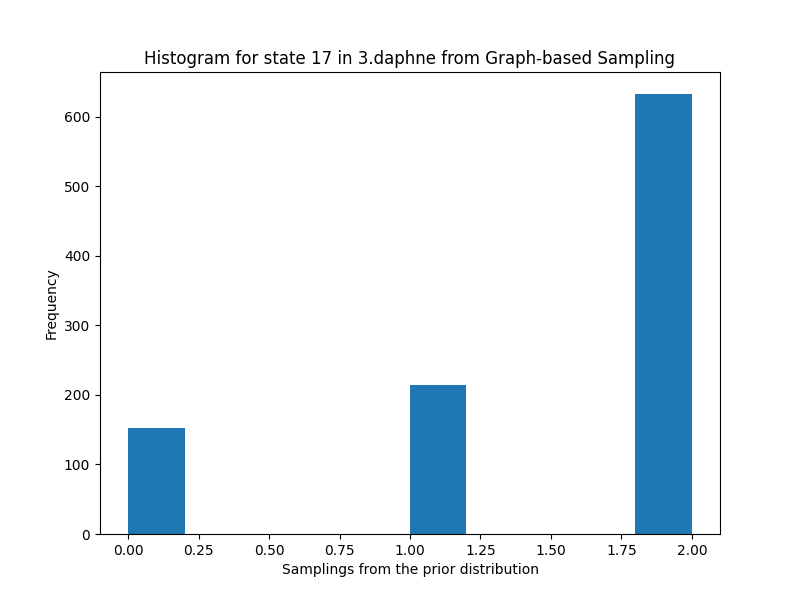
\includegraphics[width=0.24\textwidth]{../figs/graph_3_17}%
   	  \label{fig:f}%
   	  }%
   \caption{Histograms for 3.daphne}
\end{figure}

\newpage
\item Program 4): in 1000 samplings from this program,  each return values is a 3-D array incorporating the estimations for $W_0, b_0, W_1, b_1$.  $W_0$ is a 2-D array of size $10\times 1$, $b_0$ is a 2-D array of size $10\times 1$, $W_1$ is a 2-D array of size $10\times 10$, and $b_1$ is a 2-D array of size $10\times 1$.
\begin{figure}[!htp]
	\centering
    \subfloat[Samples from the prior for $W_0$]{%
        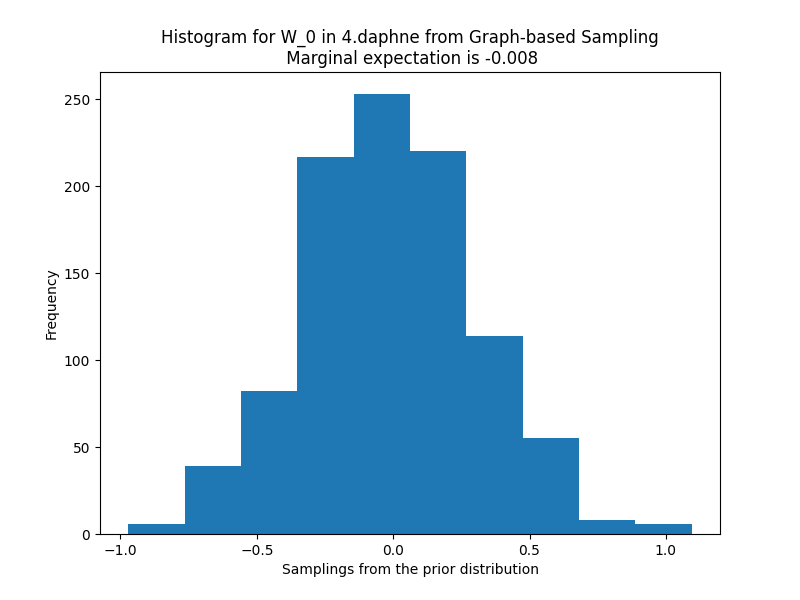
\includegraphics[width=0.4\textwidth]{../figs/graph_4_1}%
        \label{fig:a}%
        }%
    \hfill%
    \subfloat[Samples from the prior for $b_0$]{%
        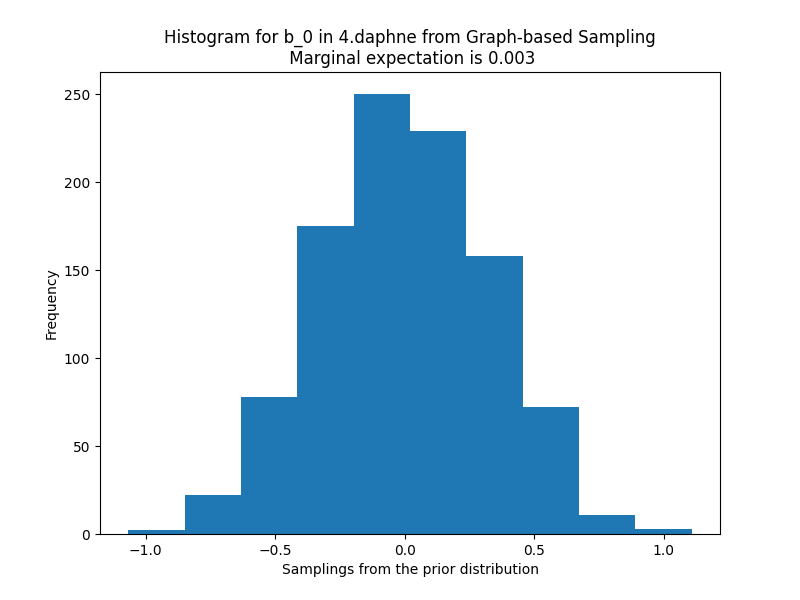
\includegraphics[width=0.4\textwidth]{../figs/graph_4_2}%%
        \label{fig:b}%
        }%
	
	\centering
    \subfloat[Samples from the prior for $W_1$]{%
        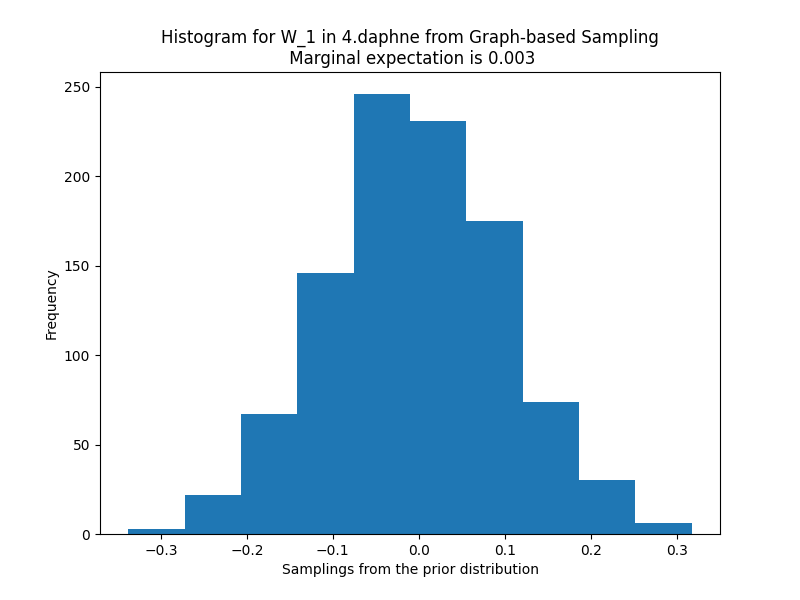
\includegraphics[width=0.4\textwidth]{../figs/graph_4_3}%
        \label{fig:a}%
        }%
    \hfill%
    \subfloat[Samples from the prior for $b_1$]{%
        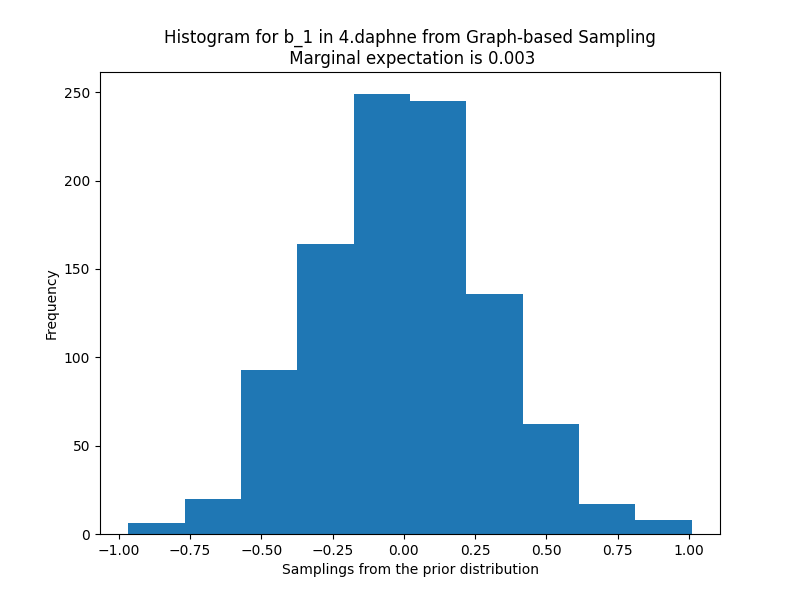
\includegraphics[width=0.4\textwidth]{../figs/graph_4_4}%%
        \label{fig:b}%
        }%
        \caption{Histograms for 4.daphne}
\end{figure}
\end{enumerate}

\newpage
\item Tests in Evaluation-based sampling.py are passed:

\begin{figure}[!htp]
	\centering
	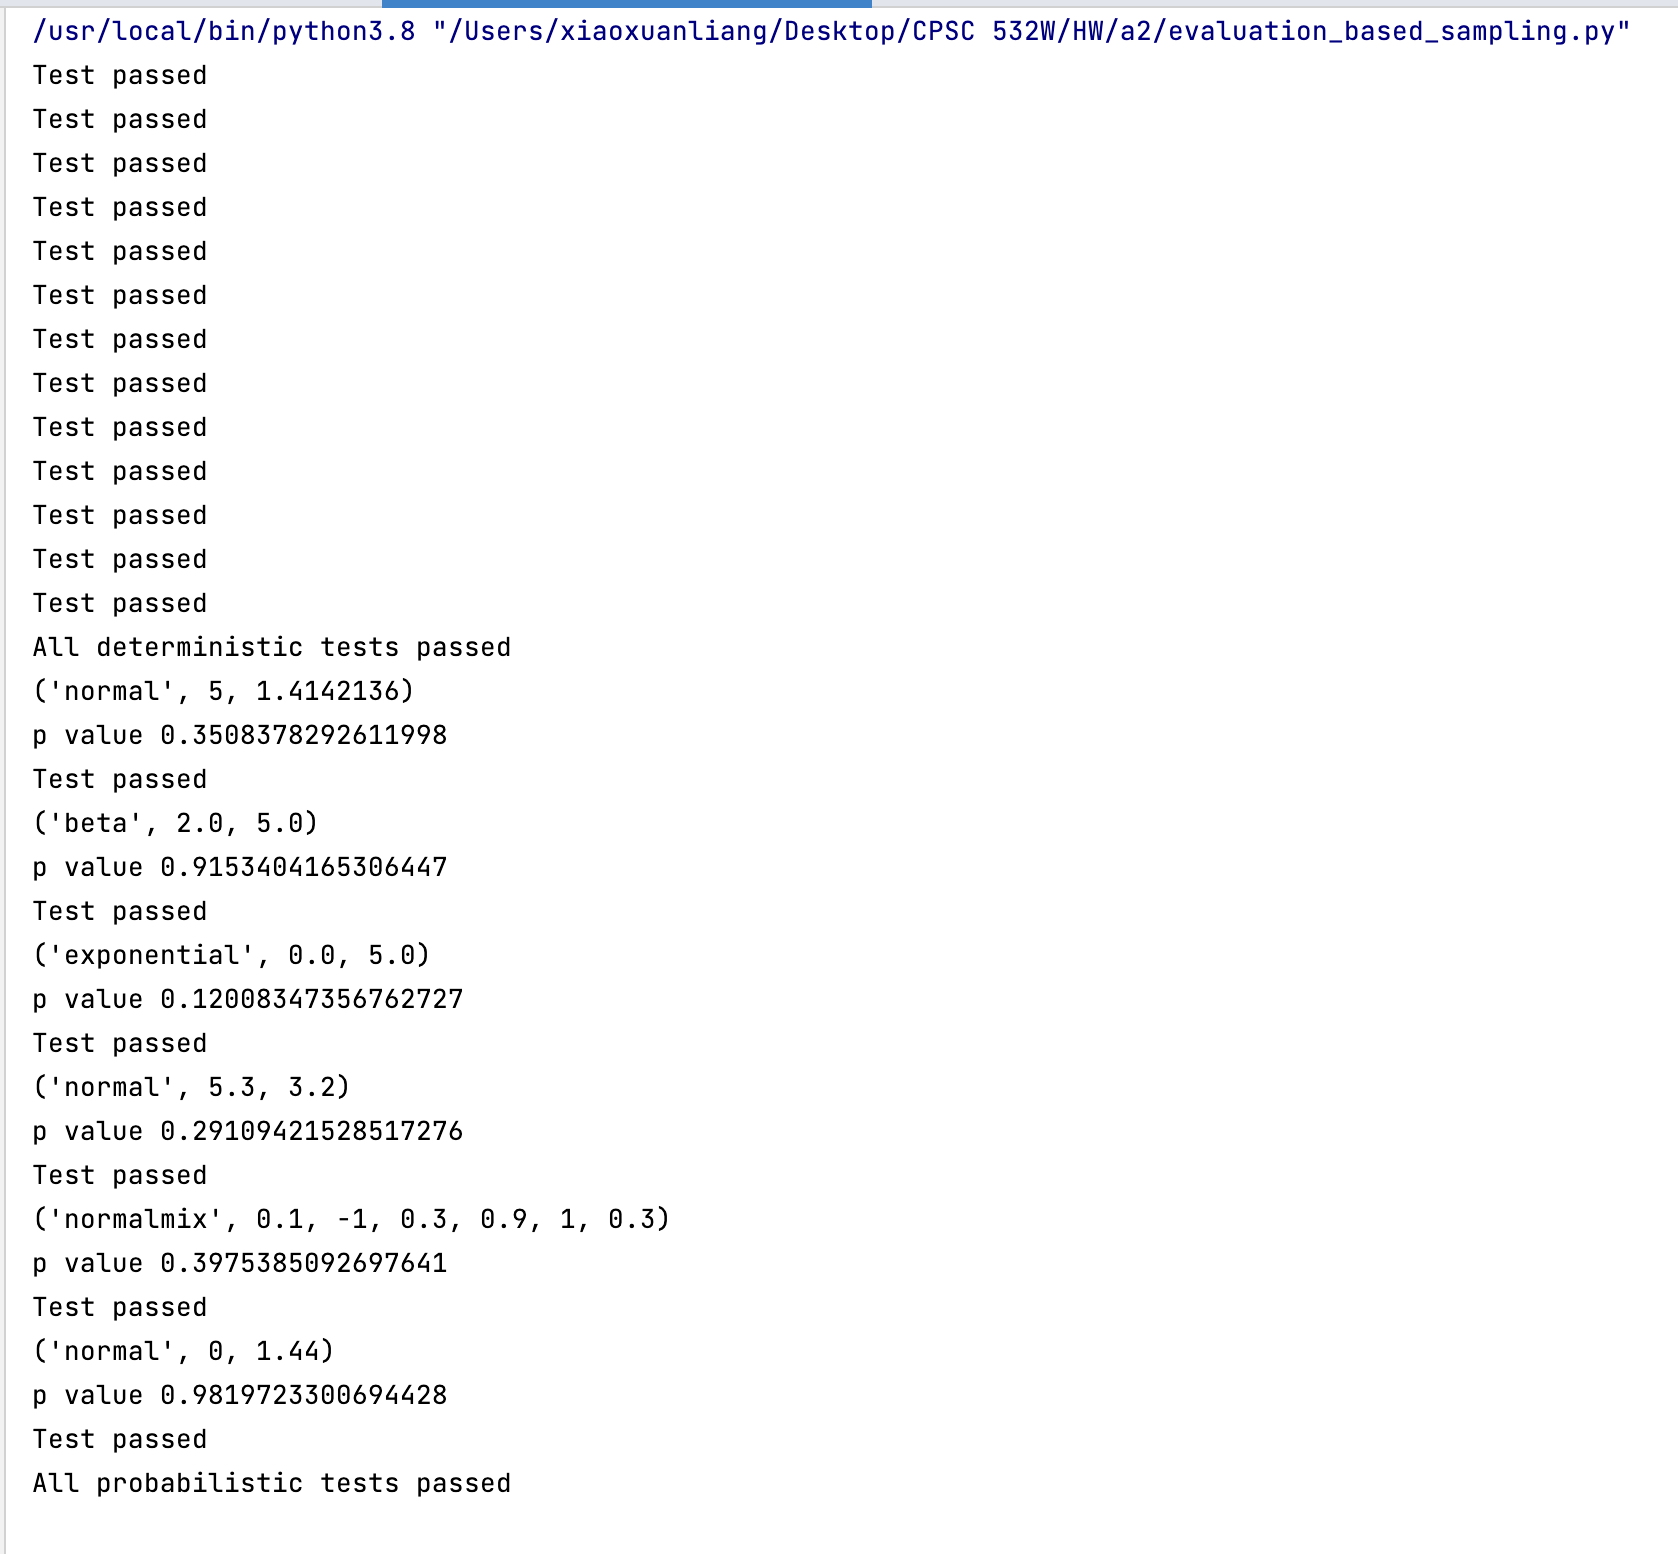
\includegraphics[scale=0.6]{../figs/evaluation_tests}
\end{figure}

\newpage
Tests in Graph-based sampling.py are passed:
\begin{figure}[!htp]
	\centering
	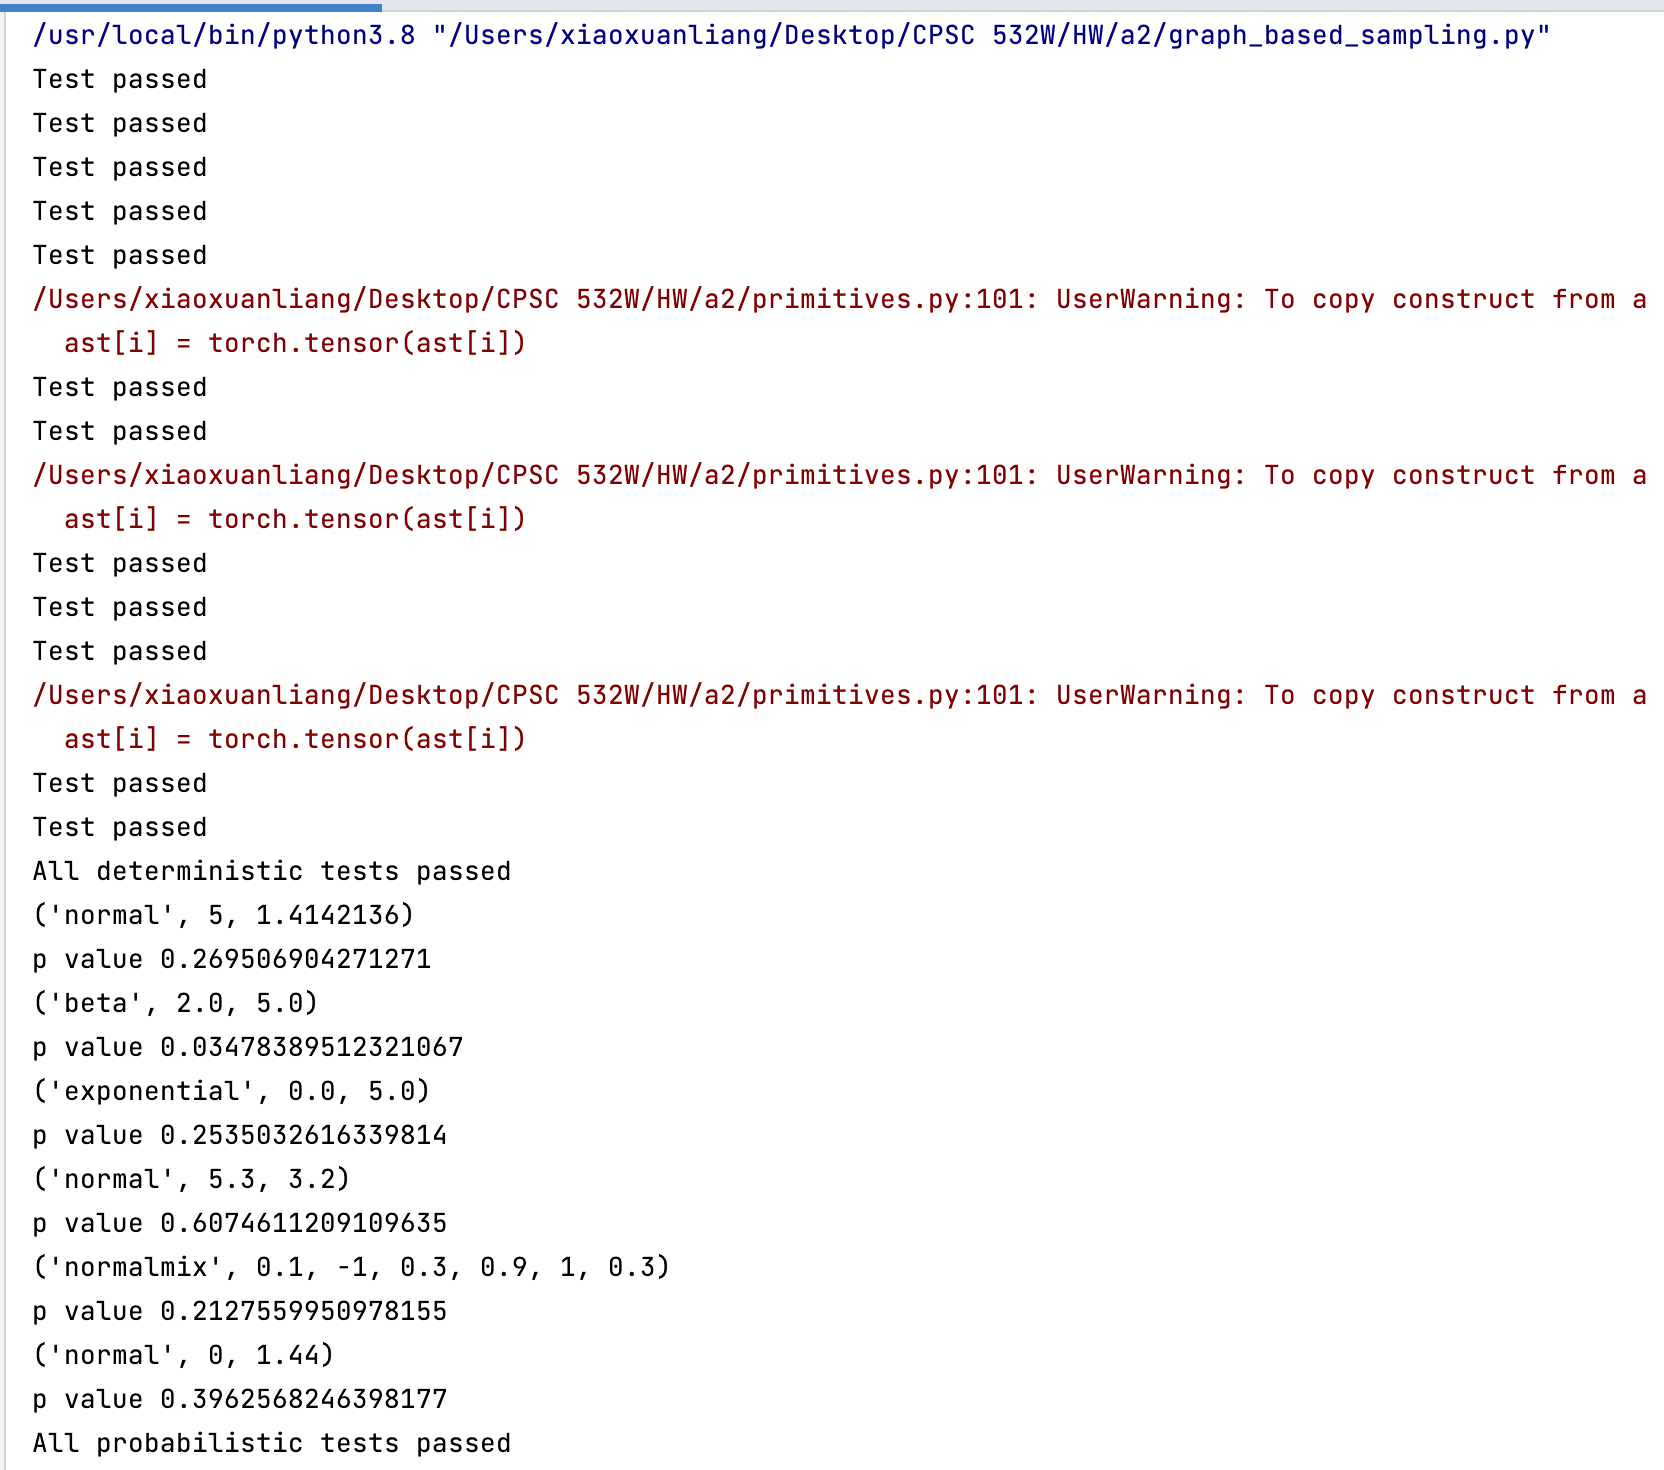
\includegraphics[scale=0.6]{../figs/graph_tests}
\end{figure}

\newpage
\item Code snippets:
Evaluation-based sampling.py:
\begin{figure}[!htp]
	\centering
	\includegraphics[scale=0.4]{../figs/evaluation_code1}
	\caption{Function evaluate_program}
\end{figure}

\begin{figure}[!htp]
	\centering
	\includegraphics[scale=0.5]{../figs/evaluation_code2}
	\caption{Helper function for evaluation_program}
\end{figure}

\begin{figure}[!htp]
	\centering
	\includegraphics[scale=0.5]{../figs/evaluation_code3}
	\caption{Helper function for evaluation_program}
\end{figure}

\newpage

Graph-based sampling.py:
\begin{figure}[!htp]
	\centering
	\includegraphics[scale=0.6]{../figs/graph_code1}
	\caption{function maps and function deterministic_eval}
\end{figure}

\begin{figure}[!htp]
	\centering
	\includegraphics[scale=0.6]{../figs/graph_code2}
	\caption{Function sample_from_joint Part I}
\end{figure}

\begin{figure}[!htp]
	\centering
	\includegraphics[scale=0.6]{../figs/graph_code3}
	\caption{Function sample_from_joint Part II}
\end{figure}

\begin{figure}
	\centering
	\includegraphics[scale=0.6]{../figs/graph_code4}
	\caption{Helper function for sample_from_joint}
\end{figure}

\newpage
Primitives.py:
\begin{figure}[!htp]
	\centering
	\includegraphics[scale=0.6]{../figs/primitive_code1}
	\caption{helper function}
\end{figure}

\begin{figure}[!htp]
	\centering
	\includegraphics[scale=0.6]{../figs/primitive_code2}
	\caption{helper function}
\end{figure}

Primitives.py:
\begin{figure}[!htp]
	\centering
	\includegraphics[scale=0.6]{../figs/primitive_code3}
	\caption{helper function}
\end{figure}
\end{enumerate}
\end{document}